\begin{frame}{Logic}

% Example de base
% Deduction
    
\vfill
\begin{itemize}
    \item With,
    \vfill
\begin{center}
\begin{tabular}{lll}
    Statement A & & All men are mortal \\
    Statement B & & Socrates is a man
\end{tabular}
\end{center}
    \vfill
    \item One can deduce,
    \vfill
\begin{center}
\begin{tabular}{lll}
    Statement C & & Socrates is mortal \\
\end{tabular}
\end{center}
\vfill \item Deduction goes from general to specific
\begin{itemize}
    \item[\ding{43}] Statement A is more 'general' than statement C
\end{itemize}
\end{itemize}
\vfill    

\end{frame}

\begin{frame}{Generality with subsumption (i)}
\vfill
\begin{block}{Formula substitution}
Let $\theta$ be a substitution of the form \{$v_1/t_1, ..., v_n/t_n$\}. \\
Let $F$ be an arbitrary formula. \\
$F\theta$ is the formula $F$ where each of its variable $v_i$ have been replaced by $t_i$.
\end{block}
\vfill
\begin{block}{Atom subsumption}
Let $\theta$ be a substitution of the form \{$v_1/t_1, ..., v_n/t_n$\}. \\
Let $F$ be an arbitrary atom. \\
$F\theta$ is the formula $F$ where each of its variable $v_i$ have been replaced by $t_i$.
\end{block}
\vfill
\begin{block}{Clause subsumption}
Let $C$ and $D$ be clauses. \\
$C \preceq D$, i.e. $C$ subsumes $D$ iff $\exists \theta, C\theta \subseteq D$.
\end{block}
\vfill
\end{frame}

\begin{frame}{Generality with subsumption (ii)}
\vfill
\begin{center}
\begin{tabular}{lllll}
    A & & All men are mortal & & mortal(X) \\
    C & & Socrates is mortal & & mortal(socrates) \\
\end{tabular}
\end{center}    
\vfill
\begin{itemize}
\item Let $\theta = \{X/\text{socrates}\}$
\begin{center}
\begin{tabular}{llll}
&$A\theta$&$=$&$C$\\
$\Leftrightarrow$&$A$&$\preceq$&$C$
\end{tabular}    
\end{center}
\vfill
    \item[\ding{43}] Statement A is indeed more general than statement C
    \vfill
\end{itemize}
\end{frame}

\begin{frame}{Generality with entailment}
\vfill
\begin{itemize}
    \item Clauses of interest:
\end{itemize}
\vfill
\begin{center}
\begin{tabular}{lll}
    A & & mortal(X) $\leftarrow$ man(X) \\
    C & & mortal(socrates) \\
\end{tabular}
\end{center}    
\vfill
\begin{itemize}
    \item Background knowledge:
    \vfill
        \begin{center}\hspace{-55pt}
        \begin{tabular}{lll}
            B & & man(socrates) \\
        \end{tabular}
        \end{center}    
\vfill
    \item $A, B \models C$
    \vfill
    \begin{itemize}
        \item[\ding{43}] With B as background knowledge, A entails C
    \end{itemize}
\end{itemize}    
\vfill
\end{frame}

\begin{frame}{Inductive logic programming (i)}
\begin{center}
\vfill
\begin{tabular}{lllll}
B && Background knowledge && Logic program \\
E && Examples && Set of ground unit clauses \\
H && Hypothesis && Logic program
\end{tabular}
\vfill
Given B and E, find H, such that:
$$ B, H \models E $$
\vfill
\end{center}
\end{frame}

\begin{frame}{Inductive logic programming (ii)}
% Shapiro's learning
\vfill
Shapiro's refinement graph:
\vfill
\begin{figure}
    \centering
    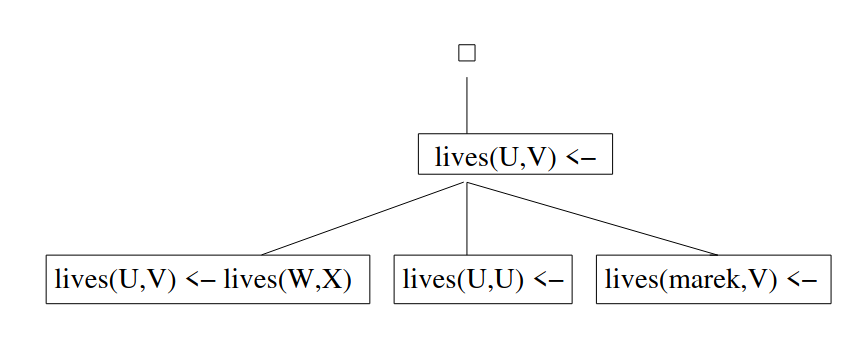
\includegraphics[width=.5\textwidth]{images/Shapiro's graph.png}
%    \caption{Caption}
%    \label{fig:my_label}
\end{figure}
\vfill
\begin{itemize}
    \item Search unbounded
    \item Consider many solution that do not entail all examples
    \item Prolog uses this type of search
\end{itemize}

\end{frame}

\begin{frame}{Inductive logic programming (iii)}
\vfill
There exists another learning approach:
\vfill
\begin{center}
    Given $B$ and $E$, find $H$, such that:
    \begin{eqnarray*}
    B, H &\models& E \\
    B, \overline{E} &\models& \overline{H} \\
    B, \overline{E} &\models& \overline{\perp} \models \overline{H}\\
    H &\models& \perp
    \end{eqnarray*}  
\end{center}
\vfill
\begin{itemize}
    \item $\overline{\perp}$ is the conjunction of literals that are true in all models $B \wedge \overline{E}$
    \item $\perp$ is the most specific clause for $B$ and $E$
    \item The algorithm explores hypotheses more general than $\perp$
    \item The algorithm uses a metric to rank hypotheses
    \begin{itemize}
        \item[\ding{43}] hypothesis chosen to be general but with few literals
    \end{itemize}
    \item Progol uses this type of search
\end{itemize}
\vfill
\end{frame}

\begin{frame}{Limitations}
\vfill
\begin{itemize}
    \item There are two main limitations to this approach:
\begin{enumerate}
    \item Cannot invent predicates
    \item Does not handle recursion
\end{enumerate}
\vfill    
\item Those two limitations are handled by meta interpretative learning (MIL)
\vfill
\end{itemize}
\end{frame}

\begin{frame}{Context free grammar}
\begin{itemize}
    \item A context free grammar consists of production rules of the following form:
    \begin{eqnarray*}
    S &\rightarrow& \lambda \\   
    S &\rightarrow& aS \\   
    S &\rightarrow& Sb \\   
    S &\rightarrow& S_1S_2 \\   
    \end{eqnarray*}
    where $S$, $S_1$ and $S_2$ are non-terminal symbols, $a,b$ are terminal symbols and $\lambda$ marks the end of the string
\end{itemize}
\end{frame}

\begin{frame}{Meta interpretative learning (i)}
\begin{itemize}
    \item Parity example:
\end{itemize}
\begin{figure}
    \centering
    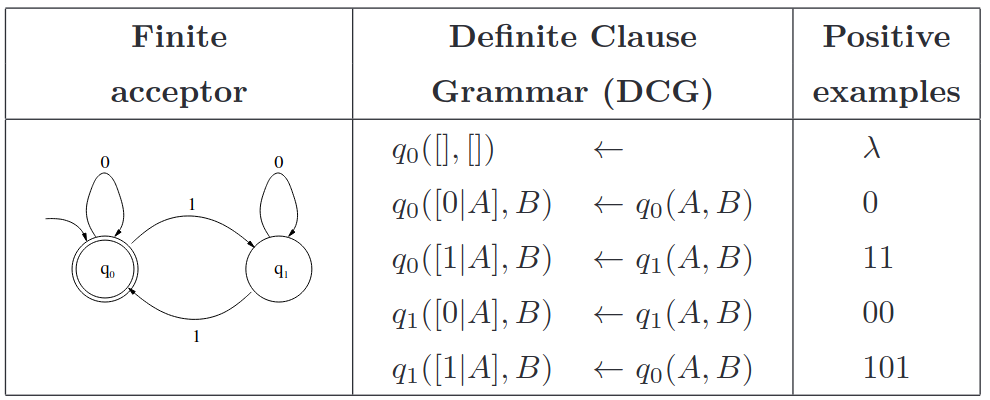
\includegraphics[width = 0.7\textwidth]{images/parity schema.png}
\end{figure}
\begin{itemize}
\item The example above allow only strings containing an even number of ones 
\item How do we learn such a model from examples?
\end{itemize}
\end{frame}

\begin{frame}{Meta interpretative learning (ii)}
\begin{itemize}
    \item Parity example:
\end{itemize}
\begin{figure}
    \centering
    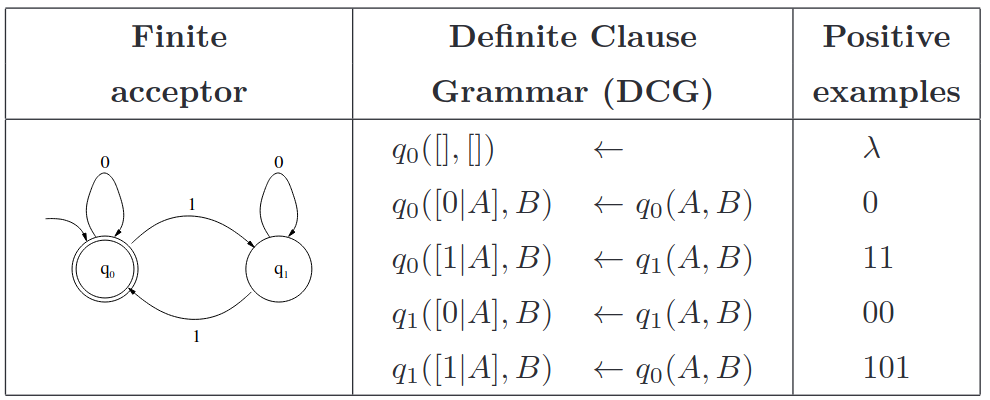
\includegraphics[width = 0.7\textwidth]{images/parity schema.png}
\end{figure}
\begin{itemize}
\item Observe that clauses take the form
\begin{eqnarray*}
Q([],[]) &\leftarrow& \\
Q([C|x],y) &\leftarrow& Q(x,y)
\end{eqnarray*}
\end{itemize}
\end{frame}

\begin{frame}{Meta interpretative learning (iii)}
\vfill
\begin{eqnarray*}
Q([],[]) &\leftarrow& \\
Q([C|x],y) &\leftarrow& Q(x,y)
\end{eqnarray*}
\vfill
\begin{figure}
    \centering
    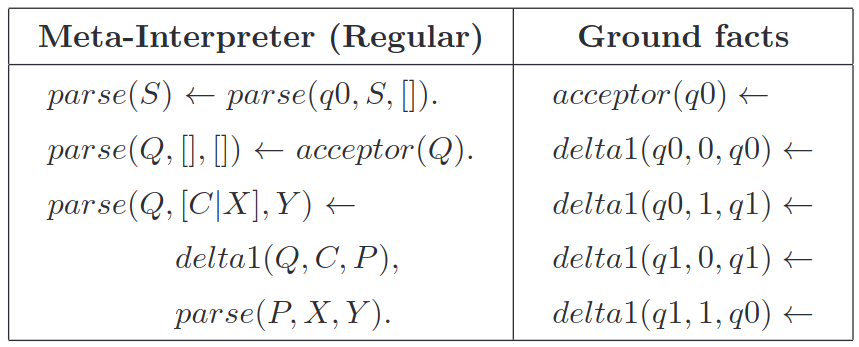
\includegraphics[width=.7\textwidth]{images/metainterpret.png}
\end{figure}    
\vfill
\begin{itemize}
    \item Using the new formulation, we can build an interpreter
    \item We still want to learn the ground facts from examples
\end{itemize}
\end{frame}

\begin{frame}[fragile]{Meta interpretative learning (iv)}
\vspace{-.5cm}
\begin{minted}[breaklines, bgcolor=black!10, fontsize=\scriptsize]{prolog}
% Meta interpretor for regular grammar
parse(S,G1,G2) :- parse(s(0),S,[],G1,G2).

parse(Q,X,X,G1,G2) :- abduce(acceptor(Q),G1,G2).
parse(Q,[C|X],Y,G1,G2) :- skolem(P), abduce(delta1(Q,C,P),G1,G3), parse(P,X,Y,G3,G2).

abduce(X,G,G) :- member(X,G).
abduce(X,G,[X|G]) :- not(member(X,G)).

skolem(s(0)). skolem(s(1)).

% Examples for parity example
parse([],[],G1), parse([0],G1,G2), parse([0,0],G2,G3), parse([1,1],G3,G4), parse([0,0,0],G4,G5), parse([0,1,1],G5,G6), parse([1,0,1],G6,G), not(parse([1],G,G)), not(parse([0,1],G,G).

% Output
G = [delta1(s(1),0,s(1)), delta1(s(0),1,s(1)), delta1(s(1),1,s(0)), delta1(s(0),0,s(0)), acceptor(s(0))]
\end{minted}
\vspace{-.6cm}
\begin{itemize}
    \item In a few lines of Prolog, we can quickly learn the parity example
    \item This model is called Metagol$_R$
\end{itemize}
\end{frame}

\begin{frame}[fragile]{Learning in action}
\begin{minted}[breaklines, bgcolor=black!10]{prolog}
% Meta interpretor for regular grammar
parse(S,G1,G2) :- parse(s(0),S,[],G1,G2).

parse(Q,X,X,G1,G2) :- abduce(acceptor(Q),G1,G2).
parse(Q,[C|X],Y,G1,G2) :- skolem(P), abduce(delta1(Q,C,P),G1,G3), parse(P,X,Y,G3,G2).

abduce(X,G,G) :- member(X,G).
abduce(X,G,[X|G]) :- not(member(X,G)).

skolem(s(0)). skolem(s(1)).
\end{minted}    

\vfill

\only<1>{ 
\mintinline{prolog}{? parse([],[],G1).} \\
\mintinline{prolog}{H = []}
}

\only<2>{ 
\mintinline{prolog}{? parse(s(0),[],[],[],G1).} \\
\mintinline{prolog}{H = []}
}

\only<3>{ 
\mintinline{prolog}{? abduce(acceptor(s(0)),[],G1).} \\
\mintinline{prolog}{H = []}
}

\only<4>{ 
\mintinline{prolog}{G1 = [acceptor(s(0))])} \\
\mintinline{prolog}{H = G1 = [acceptor(s(0))]}
}

\only<5>{ 
\mintinline{prolog}{? parse([0],[acceptor(s(0))],G2).} \\
\mintinline{prolog}{H = [acceptor(s(0))]}
}

\only<6>{ 
\mintinline{prolog}{? parse(s(0),[0],[],[acceptor(s(0))],G2).} \\
\mintinline{prolog}{H = [acceptor(s(0))]}
}

\only<7>{ 
\mintinline{prolog}{? skolem(P), abduce(delta1(s(0),0,P),[acceptor(s(0))],T),}\\ \mintinline{prolog}{| parse(P,[],[],T,G2).} \\
\mintinline{prolog}{H = [acceptor(s(0))]}
}

\only<8>{ 
\mintinline{prolog}{? abduce(delta1(s(0),0,s(0)),[acceptor(s(0))],T),}\\ \mintinline{prolog}{| parse(s(0),[],[],T,G2).} \\
\mintinline{prolog}{H = [acceptor(s(0))]}
}

\only<9>{ 
\mintinline{prolog}{? parse(s(0),[],[],[delta1(s(0),0,s(0)), acceptor(s(0))],G2).} \\
\mintinline{prolog}{H = [acceptor(s(0))]}
}

\only<10>{ 
\mintinline{prolog}{? abduce(acceptor(s(0)),}
\mintinline{prolog}{| [delta1(s(0),0,s(0)), acceptor(s(0))],G2).} \\
\mintinline{prolog}{H = [acceptor(s(0))]}
}

\only<11>{ 
\mintinline{prolog}{G2 = [delta1(s(0),0,s(0)), acceptor(s(0))]} \\
\mintinline{prolog}{H = G2 = [delta1(s(0),0,s(0)), acceptor(s(0))]}
}
\end{frame}

\begin{frame}{Meta interpretative learning (v)}
\begin{itemize}
    \item MIL has gone even further to consider other metarules
    \begin{figure}
        \centering
        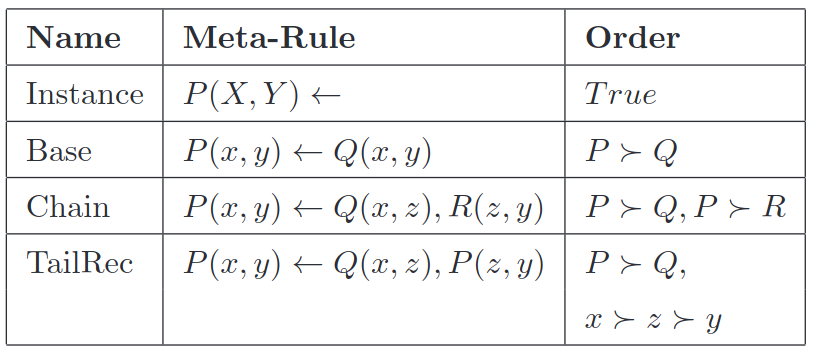
\includegraphics[width=.6\textwidth]{images/newmetarules.png}
    \end{figure}
    \item It considers datalog logic programs in $\mathcal{H}_2^2$
    \begin{itemize}
        \item arity $\leq2$ for predicates
        \item \#atoms $\leq2$ in the body of clauses
    \end{itemize}
    \item $\mathcal{H}_2^2$ has Universal Turing Machine expressivity
\end{itemize}    
\end{frame}

\begin{frame}{ILP for texts of law}
\vfill
\begin{itemize}
    \item There are at least three ways to study texts of law with ILP
    \begin{itemize}
\vfill
        \item[\ding{43}] Identify logical rules in texts of law and generalize them with ILP (slides 6-8)
\vfill
        \item[\ding{43}] Suppose that words in texts of law form a context free grammar and learn it with MIL (slides 11-14)
\vfill
        \item[\ding{43}] Believe in the expressivity of $\mathcal{H}_2^2$ (slide 15)
    \end{itemize}
\end{itemize}
    \vfill

\end{frame}